\chapter{Theoretical Background}%
\label{cha:background}

This chapter will give an overview of the theoretical background of the problem
investigated in this thesis, as well as the methods used. We will first
introduce the topic of outliers on an intuitive level and then try to highlight
a more rigorous approach. We will move on to introduce neural network models
especially in their invertible variant and how specific training schemes are
particularly useful for investigating outliers. Finally we will introduce
archetypal analysis as a general concept and also as an add-on to more
complicated models.


\section{Outliers And Outlier Detection}%
\label{sec:outliers_an_outlier_detection}

% - outliers are task specific, subjective
% - methods of outlier detection
%     - typicality
%     - research more methods


\section{Invertible Neural Networks}% Generative Models?
\label{sec:invertible_neural_networks}

% - Neural Networks and their importance (briefly)
Neural networks and deep learning methods have become staple methods in many
fields that use machine learning. They are typically comprised of a chain of relatively
simple, non-linear blocks.~\citep{lecunDeepLearning2015}

As representation-learning methods, neural networks have found use for
many discriminative as well as generative tasks. Especially in recent years
many advance were made for generative methods using neural networks. One such
advancement was the introduction of invertible neural networks. Neural
networks, though not invertible in general, can be made fully invertible by
cleverly designing its building blocks to be invertible.
% invertible -> bijective?

We will now briefly introduce two other generative models based on neural networks
before introducing invertible neural networks in detail.

\paragraph{Generative Adversarial Networks}%
\label{par:generative_adversarial_networks}

\paragraph{Variational Autoencoders}%
\label{par:variational_autoencoders}

\subsection{Coupling Layers}%
\label{sub:coupling_layers}

In general, neural networks are composed of multiple layers or composite
functions. The function $\mathcal{F}$ a neural network with $L$ layers computes
is given by
\begin{equation}%
    \label{eq:neural_network}
    \mathcal{F} = f_L \circ \dots \circ f_2 \circ f_1
\end{equation}

If we design all layers to be bijective and have tractable Jacobian determinant the whole
forward computation is invertible by composing the inverse layers in reverse
order.
\begin{equation}%
    \label{eq:neural_network_inv}
    \mathcal{F}^{-1} = f_L^{-1} \circ \dots \circ f_2^{-1} \circ f_1^{-1}
\end{equation}

Dinh et al.\ \citep{dinhNICENonlinearIndependent2015} describe a family of transformations
called coupling layers, that can be used as components in a invertible neural
network. In general, coupling layers are defined as follows

\begin{definition}[General Coupling Layer]
    Let $x \in \mathcal{X}$, the input to the layer, be a vector in $\mathbb{R}^D$
    and $I_1, I_2$ a partition of $[1, D]$ such that $d = |I_1|$ and $m$ a
    function defined on $\mathbb{R}^d$. We can then define $y = (y_{I_1},
    y_{I_2})$ as
    \begin{equation}
        \begin{aligned}%
            \label{eq:coupling_layer_transform}
            y_{I_1} &= x_{I_1} \\
            y_{I_2} &= g(x_{I_2};m(x_{I_1}))
        \end{aligned}
    \end{equation}
    where $g: \mathbb{R}^{D-d} \times m(\mathbb{R}^d) \rightarrow
    \mathbb{R}^{D-d}$ is the coupling law, an invertible map with respect to
    the first argument given its second. This transformation is called coupling
    layer with coupling function $m$.
\end{definition}

Note that the choice of $m$ is not constrained to invertible functions but can
be arbitrary.

% TODO: Additive coupling layer, volume preserving %
A simple choice for the coupling law would be an additive law
~\citep{dinhNICENonlinearIndependent2015, gomezReversibleResidualNetwork2017}.
The coupling layer transformation then becomes
\begin{equation}
    \begin{aligned}%
        \label{eq:add_coupling_transform}
        y_{I_1} &= x_{I_1} \\
        y_{I_2} &= x_{I_2} + m(x_{I_1})
    \end{aligned}
\end{equation}
This transformation has unit Jacobian determinant, i.e.\ is volume preserving.
This can give numerical stability especially if $m$ is a rectified linear
network. This however comes at the cost of what transformations can be learned.

\begin{figure}[htpb]
    \centering
    \begin{subfigure}[t]{0.8\textwidth}
        \centering
        \begin{tikzpicture}
            \node[varnode] (x1)                   {$x_{I_1}$};
            \node[connectnode] (c1)   [right=0.5cm of x1]    {};
            \node[varnode] (y1) [right=5cm of x1] {$y_{I_1}$};
            \node[varnode] (x2) [below=2.5cm of x1] {$x_{I_2}$};
            \node[varnode] (y2) [right=5cm of x2] {$y_{I_2}$};
            \node[opnode] (plus) [right=3.0cm of x2] {$+$};
            \node[opnode] (m) at ($(c1)!2cm!(plus)$) {$m$};


            \draw[grapharrow] (x1) -- (y1);
            \draw[grapharrow] (c1) -- (m);
            \draw[grapharrow] (x2) -- (plus);
            \draw[grapharrow] (m) -- (plus);
            \draw[grapharrow] (plus) -- (y2);
        \end{tikzpicture}
    \end{subfigure}
    \par\bigskip
    \begin{subfigure}[b]{0.8\textwidth}
        \centering
        \begin{tikzpicture}
            \node[varnode] (x1)                   {$x_{I_1}$};
            \node[varnode] (y1) [right=5cm of x1] {$y_{I_1}$};
            \node[connectnode] (c1)   [left=0.5cm of y1]    {};
            \node[varnode] (x2) [below=2.5cm of x1] {$x_{I_2}$};
            \node[varnode] (y2) [right=5cm of x2] {$y_{I_2}$};
            \node[opnode] (plus) [left=3.0cm of y2] {$-$};
            \node[opnode] (m) at ($(c1)!2cm!(plus)$) {$m$};


            \draw[grapharrow] (y1) -- (x1);
            \draw[grapharrow] (c1) -- (m);
            \draw[grapharrow] (y2) -- (plus);
            \draw[grapharrow] (m) -- (plus);
            \draw[grapharrow] (plus) -- (x2);
        \end{tikzpicture}
    \end{subfigure}
\caption{Additive coupling block. Left: forward computation, right: inverse
computation.}%
\label{fig:additive_coupling_block}
\end{figure}

% TODO: GLOW coupling blocks %
A more versatile approach is to use affine coupling blocks, that allow for
non-volume preserving transformations. The coupling layer transformation for
the general affine coupling block introduced by Dinh et
al.~\citep{dinhDensityEstimationUsing2017} is
\begin{equation}
    \begin{aligned}%
        \label{eq:affine_coupling_transform}
        y_{I_1} &= x_{I_1} \\
        y_{I_2} &= x_{I_2} \odot \exp ( s(x_{I_1})) + t(x_{I_1})
    \end{aligned}
\end{equation}
where $s$ and $t$ are arbitrary functions that map $\mathbb{R}^{D-d}
\rightarrow \mathbb{R}^d$ and stand for scale and translation respectively and
$\odot$ is the Hadarmat or pointwise product.
This transformation is again easily invertible, regardless of the complexity of
$s$ and $t$
\begin{equation}
    \begin{aligned}%
        \label{eq:inv_affine_coupling_transform}
        x_{I_1} &= y_{I_1} \\
        x_{I_2} &= (y_{I_2} - t(y_{I_1})) \odot \exp (-s(y_{I_1}))
    \end{aligned}
\end{equation}

\begin{figure}[htpb]
\begin{center}
    \begin{subfigure}[b]{0.8\textwidth}
        \centering
        \begin{tikzpicture}
            \node[varnode]     (x1)                          {$x_{I_1}$};
            \node[connectnode] (c1)   [right=0.5cm of x1]    {};
            \node[connectnode] (c2)   [right=1.7cm of x1]    {};
            \node[varnode]     (y1)   [right=5cm   of x1]    {$y_{I_1}$};
            \node[varnode]     (x2)   [below=2.5cm of x1]    {$x_{I_2}$};
            \node[varnode]     (y2)   [right=5cm   of x2]    {$y_{I_2}$};
            \node[opnode]      (plus) [right=1.5cm of x2]    {$+$};
            \node[opnode]      (mul)  [right=2.7cm of x2]    {$\times$};
            \node[opnode]      (t)    at ($(c1)!2cm!(plus)$) {$t$};
            \node[opnode]      (s)    at ($(c2)!2cm!(mul)$)  {$s$};


            \draw[grapharrow] (x1)   -- (y1);
            \draw[grapharrow] (c1)   -- (t);
            \draw[grapharrow] (c2)   -- (s);
            \draw[grapharrow] (x2)   -- (plus);
            \draw[grapharrow] (t)    -- (plus);
            \draw[grapharrow] (s)    -- (mul);
            \draw[grapharrow] (plus) -- (mul);
            \draw[grapharrow] (mul)  -- (y2);
        \end{tikzpicture}
    \end{subfigure}
    \par\bigskip
    \begin{subfigure}[b]{0.8\textwidth}
        \centering
        \begin{tikzpicture}
            \node[varnode]     (x1)                          {$x_{I_1}$};
            \node[varnode]     (y1)   [right=5cm   of x1]    {$y_{I_1}$};
            \node[connectnode] (c1)   [left=0.5cm of y1]    {};
            \node[connectnode] (c2)   [left=1.7cm of y1]    {};
            \node[varnode]     (x2)   [below=2.5cm of x1]    {$x_{I_2}$};
            \node[varnode]     (y2)   [right=5cm   of x2]    {$y_{I_2}$};
            \node[opnode]      (plus) [left=1.5cm of y2]    {$-$};
            \node[opnode]      (mul)  [left=2.7cm of y2]    {$\div$};
            \node[opnode]      (t)    at ($(c1)!2cm!(plus)$) {$t$};
            \node[opnode]      (s)    at ($(c2)!2cm!(mul)$)  {$s$};


            \draw[grapharrow] (y1)   -- (x1);
            \draw[grapharrow] (c1)   -- (t);
            \draw[grapharrow] (c2)   -- (s);
            \draw[grapharrow] (y2)   -- (plus);
            \draw[grapharrow] (t)    -- (plus);
            \draw[grapharrow] (s)    -- (mul);
            \draw[grapharrow] (plus) -- (mul);
            \draw[grapharrow] (mul)  -- (x2);
        \end{tikzpicture}
    \end{subfigure}
\end{center}
\caption{Affine coupling block. Left: forward computation, right: inverse
computation.}%
\label{fig:affine_coupling_block}
\end{figure}

To ensure all inputs are used we need to use at least two coupling blocks and
switch $x_{I_1}$ and $x_{I_2}$ between them.

% TODO: IRevNetDownsampling and permute layers %
\subsection{Downsampling}%
\label{sub:downsampling}

\begin{figure}[htpb]
\begin{center}
\begin{tikzpicture}
    \foreach \x in {0,...,2}
    \foreach \y in {0,...,2}
    {
        \node [square,draw,fill=gray!40,minimum size=1cm] (\x\y) at (2cm*\x,2cm*\y) {};
        \node [square,draw,fill=red!40,minimum size=1cm] (\x\y) at (1cm+2cm*\x,2cm*\y) {};
        \node [square,draw,fill=blue!40,minimum size=1cm] (\x\y) at (2cm*\x,1cm+2cm*\y) {};
        \node [square,draw,fill=green!40,minimum size=1cm] (\x\y) at (1cm+2cm*\x,1cm+2cm*\y) {};
    }

    \foreach \x in {0,...,2}
    \foreach \y in {0,...,2}
    {
        \node [square,draw,fill=gray!40,minimum size=1cm] (\x\y) at
            (10cm+1cm*\x,2cm+1cm*\y) {};
    }

    \foreach \x in {0,...,2}
    \foreach \y in {0,...,2}
    {
        \node [square,draw,fill=red!40,minimum size=1cm] (\x\y) at
            (9.66cm+1cm*\x,1.66cm+1cm*\y) {};
    }

    \foreach \x in {0,...,2}
    \foreach \y in {0,...,2}
    {
        \node [square,draw,fill=blue!40,minimum size=1cm] (\x\y) at
            (9.33cm+1cm*\x,1.33cm+1cm*\y) {};
    }

    \foreach \x in {0,...,2}
    \foreach \y in {0,...,2}
    {
        \node [square,draw,fill=green!40,minimum size=1cm] (\x\y) at
            (9cm+1cm*\x,1cm+1cm*\y) {};
    }

    \draw[{Straight Barb}-{Straight Barb},line width=1mm] (6cm,2.5cm) -- (8cm,2.5cm);
\end{tikzpicture}
\end{center}
\caption{IRevNet Downsampling, figure adapted from Gomez et al.~\citep{gomezReversibleResidualNetwork2017}}%
\label{fig:downsampling}
\end{figure}

In typical deep learning architectures, especially in the field of computer
vision, the inputs are downsampled in the network. This is usually done with
strided convolutions, maximum or average pooling. Since these operations entail
a loss of information they are not bijective and cannot be used in an
invertible neural network architecture, at least outside of coupling functions.
To still be able to increase field of vision of convolutions and decrease the
amount of computations in later layers different strategies can be used. Gomez
et al. used a pixel shuffle operation, where spatial dimensions are reduce and
shifted into channel dimensions as shown
in~\autoref{fig:downsampling}~\citep{gomezReversibleResidualNetwork2017}. 

A strategy to reduce the amount of computations done in deeper layers data can
simply be split of. The part that is split of can than be trained to resemble
noise while the other part continues through coupling layers. Towards the end
of the network the split parts are concatenated back together.


\subsection{Normalizing Flows}%
\label{sub:normalizing_flows}

% TODO: Figure latent space x -> z
\begin{figure}[htpb]
    \centering
    \begin{tikzpicture}
        \node [] (a) at (0,0) {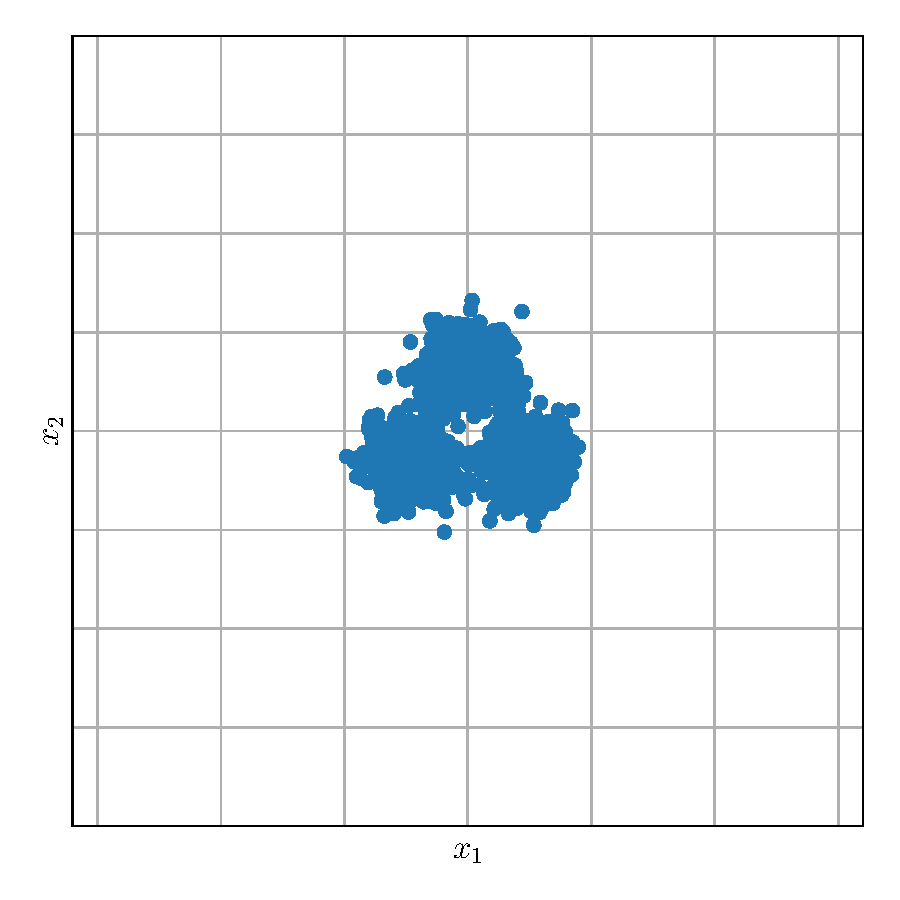
\includegraphics[width=0.3\linewidth]{figures/toy_example/gaussian_mixture/samples_grid.pdf}};
        \node [] (b) [right=of a] {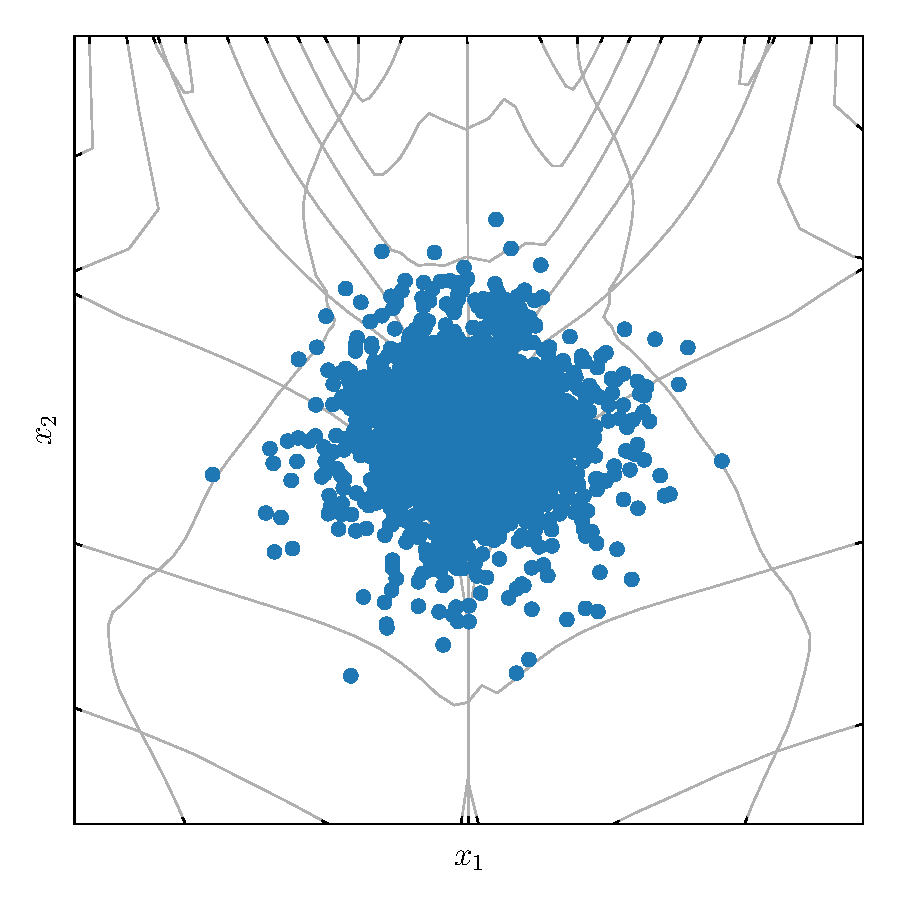
\includegraphics[width=0.3\linewidth]{figures/toy_example/gaussian_mixture/latent_grid_transformed.pdf}};
        \node [] (c) [below=of a] {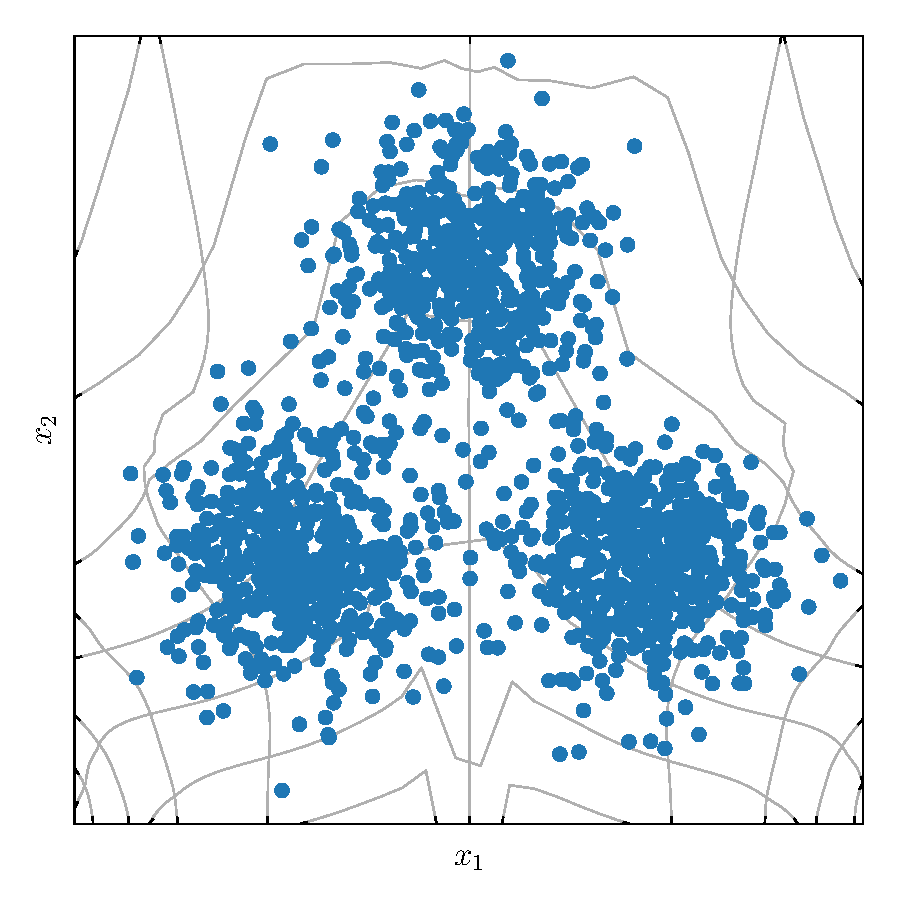
\includegraphics[width=0.3\linewidth]{figures/toy_example/gaussian_mixture/samples_grid_transformed.pdf}};
        \node [] (d) [right=of c] {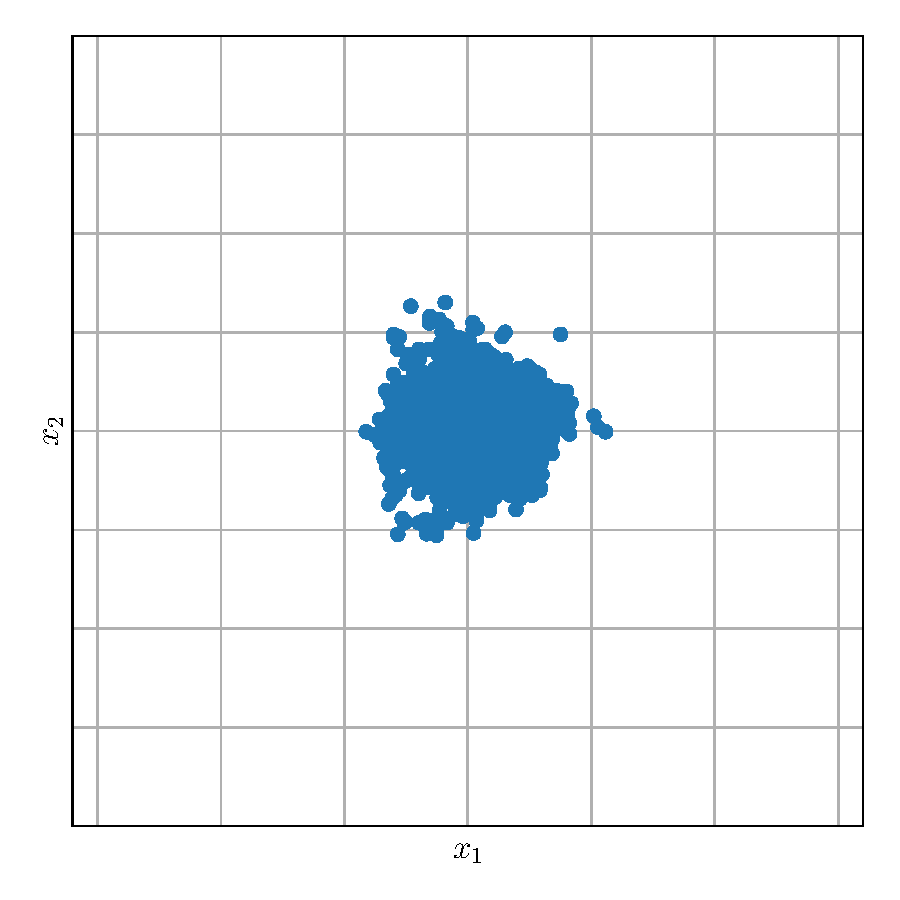
\includegraphics[width=0.3\linewidth]{figures/toy_example/gaussian_mixture/latent_grid.pdf}};
        \draw[-{Straight Barb},line width=1mm] (a) -- (b);
        \draw[{Straight Barb}-,line width=1mm] (c) -- (d);
    \end{tikzpicture}
    \caption{Mapping between data and latent space}%
    \label{fig:}
\end{figure}

Normalizing flows transform a simple probability distributions, such as a
standard normal distribution, into a complex, often intractable probability
distribution~\citep{kobyzevNormalizingFlowsIntroduction2020}. They are composed
of a series of invertible transformations, e.g. the coupling layers we defined
above. The complex probability distribution can be evaluated on a sample by
transforming it back to the simple distribution and using the change of
variables formula.

In more mathematical terms, consider vectors $\mathbf{z}_i \in \mathbb{R}^d$
that are distributed according to a simple distribution $p_{\mathbf{z}}:
\mathbb{R}^d \rightarrow \mathbb{R}$. Let $\mathcal{F}: \mathbb{R}^d
\rightarrow \mathbb{R}^d$ be an invertible transformation (e.g. an invertible
neural network). The probability density function of a variable $\mathbf{x}_i =
\mathcal{F} (\mathbf{z}_i)$ can then be computed according to the change of
variables formula
\begin{equation}%
    \label{eq:change_of_variables}
    p_{\mathbf{x}}(\mathbf{x}_i) =
    p_{\mathbf{z}}(\mathcal{F}^{-1}(\mathbf{x}_i)) \lvert J_{\mathbf{x}} \rvert^{-1}
\end{equation}
where
\begin{equation}%
    \label{eq:jacobian_det}
    J_{\mathbf{x}} = \det \frac{\partial \mathcal{F}^{-1} (\mathbf{x})}{\partial \mathbf{x}}
\end{equation}
is the Jacobian determinant of the transformation. Particularly, if
$\mathcal{F}$ is defined as in~\autoref{eq:neural_network}, the Jacobian is
simply
\begin{equation}%
    \label{eq:jacobian_chain_rule}
    J_{\mathbf{x}} = \prod \det \frac{\partial f_i^{-1} (\mathbf{x})}{\partial \mathbf{x}}
\end{equation}

To train a neural network as a normalizing flow we can simply maximize the
log-likelihood of data samples, or equivalently minimize the negative
log-likelihood. If $p_{\mathbf{z}}$ is the standard normal
distribution, the negative log-likelihood loss for a mini-batch of size $N$ can
be simply calculated as
% TODO: Check this again
\begin{equation}%
    \label{eq:nll_loss}
    \mathrm{NLL} = \frac{1}{N} \sum_i \lVert \mathcal{F}^{-1} (\mathbf{x}_i) \rVert^2 - \log J_{\mathbf{x}}
\end{equation}


\section{Archetypal Analysis}%
\label{sec:archetypal_analysis}
